% !TEX program = xelatex
\documentclass[12pt, a4paper]{ctexart}

\usepackage{amsmath, amssymb}
\usepackage{graphicx}
\usepackage{booktabs}
\usepackage{array}
\usepackage{caption}
\usepackage{geometry}
\usepackage{siunitx}
\usepackage{hyperref}

\geometry{left=2.5cm, right=2.5cm, top=2.5cm, bottom=2.5cm}
\captionsetup{font=small, labelsep=quad}
\sisetup{per-mode=symbol}

\title{\textbf{夫兰克-赫兹实验报告}\\ \large 测量氩原子的第一激发电位}
\author{}
\date{实验日期：2026 年 9 月 28 日 \quad 环境温度：\SI{25}{\celsius} \quad 仪器号：1}

\begin{document}

\maketitle

\section{实验目的}

\begin{enumerate}
    \item 测定氩（Ar）原子的第一激发电位，验证原子内部能量量子化的事实；
    \item 学习夫兰克-赫兹实验中板极电流随加速电压周期性变化的规律；
    \item 掌握用\textbf{逐差法}处理等间隔测量数据并计算物理量的方法。
\end{enumerate}

\section{实验原理}

夫兰克-赫兹管中充有低压氩气。阴极 K 发出的电子经第一栅极 $G_1$ 加速（消除阴极附近空间电荷的影响），在加速电压 $V_{G_2K}$ 作用下向第二栅极 $G_2$ 运动。若电子动能小于氩原子的第一激发能 $eU_0$，则电子与氩原子发生\textbf{弹性碰撞}，能量损失可忽略，能到达板极 A，板流 $I_A$ 随 $V_{G_2K}$ 增大而上升。当电子动能达到
\begin{equation}
    eU_0 = \frac{1}{2}mv^2
\end{equation}
时，电子与氩原子发生\textbf{非弹性碰撞}，把能量 $eU_0$ 交给氩原子使其跃迁到第一激发态，电子剩余动能很小，几乎无法克服拒斥电压 $V_{G_2A}$ 到达板极，$I_A$ 急剧下降形成\textbf{峰}。$V_{G_2K}$ 继续增大，电子在碰撞后仍保留足够动能，$I_A$ 回升；当电子在 $G_2$ 前发生第二次非弹性碰撞时，$I_A$ 再次下降形成\textbf{谷}……于是 $I_A$--$V_{G_2K}$ 曲线呈现周期性起伏。

相邻两峰（或两谷）对应的加速电压之差即氩原子的第一激发电位：
\begin{equation}
    \Delta U = U_{n+1} - U_n \approx U_0
\end{equation}
若峰位电压与峰序号 $n$ 满足线性关系 $U_n = U_1 + (n-1)\,\Delta U$，则其斜率即为 $\Delta U$。氩原子第一激发电位的参考值为 $U_0 = \SI{11.55}{eV}$。

\section{实验装置与参数}

\begin{itemize}
    \item 灯丝电压 $V_F = \SI{2.1}{V}$（恒定）
    \item 扫描范围 $V_{G_2K}$：0--\SI{80}{V}，步距 \SI{0.1}{V}，每点停留 \SI{0.5}{s}
    \item 电流量程：\SI{1}{nA}
    \item 改变第一栅压 $V_{G1K}$（1/2/\SI{3}{V}）与拒斥电压 $V_{G2A}$（7/\SI{8}{V}），共测量 6 组曲线，以研究各参量对波形的影响。各组实验条件如表~\ref{tab:groups}。
\end{itemize}

\begin{table}[htbp]
    \centering
    \caption{各组实验条件}
    \label{tab:groups}
    \begin{tabular}{ccccccc}
        \toprule
        组别 & A & B & C & D & E & F \\
        \midrule
        $V_{G1K}$ / V & 1 & 1 & 2 & 2 & 3 & 3 \\
        $V_{G2A}$ / V & 7 & 8 & 7 & 8 & 7 & 8 \\
        \bottomrule
    \end{tabular}
\end{table}

\section{实验数据与波形}

6 组 $I_A$--$V_{G_2K}$ 曲线如图~\ref{fig:curves} 所示，均呈现清晰、规则的周期性振荡，共观测到 5 个峰；波谷略滞后于峰，且随 $V_{G_2K}$ 增大峰高逐渐升高（加速电压越高，到达板极的电子越多，本底电流越大）。

\begin{figure}[htbp]
    \centering
    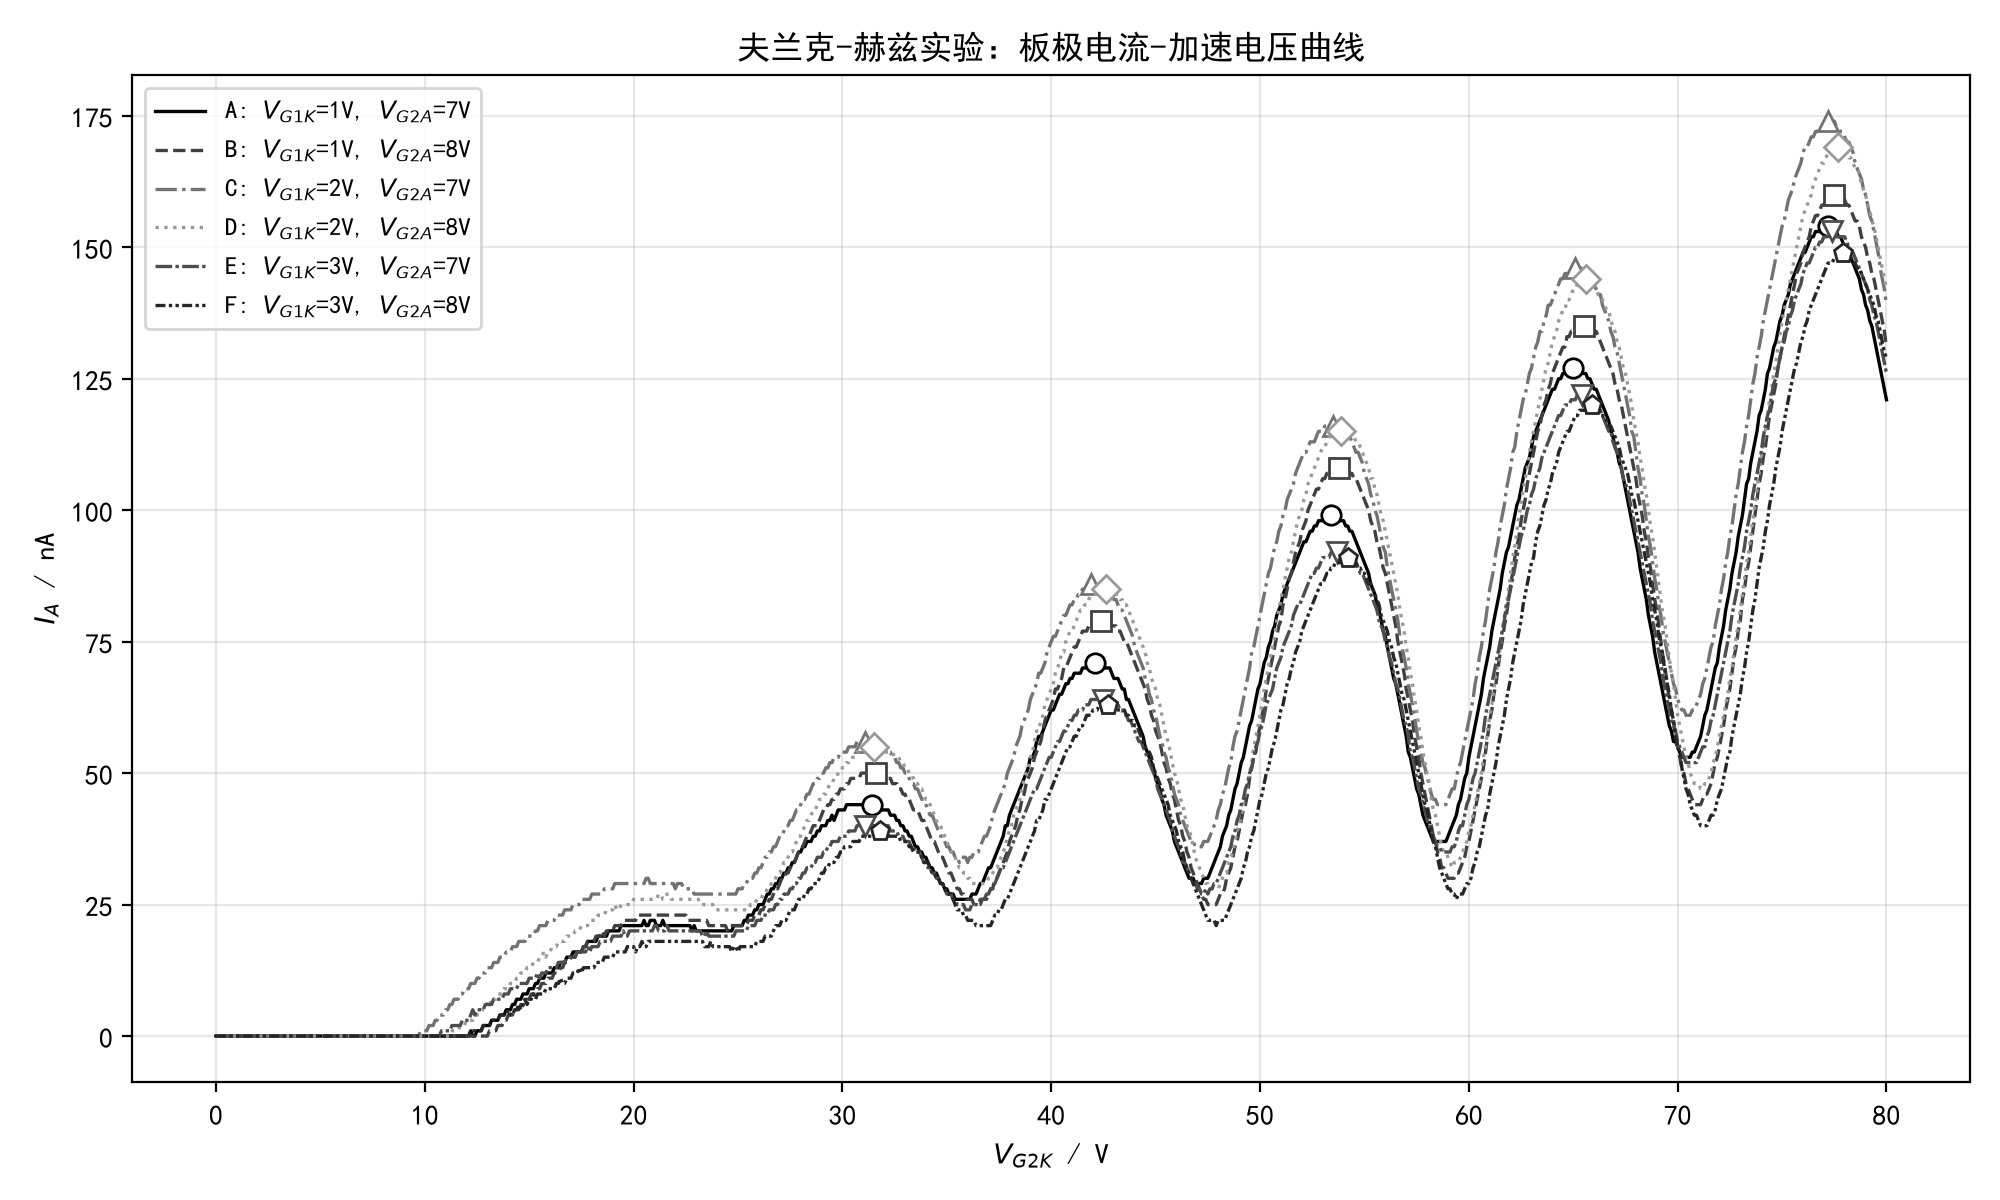
\includegraphics[width=0.9\textwidth]{frank_hertz_curves.png}
    \caption{六组实验曲线}
    \label{fig:curves}
\end{figure}

各曲线峰位电压（对数据做轻度平滑后自动寻峰，平滑仅用于定位峰位，不改变原始数据）列于表~\ref{tab:peaks}。

\begin{table}[htbp]
    \centering
    \caption{各组曲线的峰位电压（单位：V，电压读数误差 $\pm\SI{0.05}{V}$）}
    \label{tab:peaks}
    \footnotesize
    \begin{tabular}{c cccccc c}
        \toprule
        峰序号 $n$ & A(1V,7V) & B(1V,8V) & C(2V,7V) & D(2V,8V) & E(3V,7V) & F(3V,8V) & 平均 \\
        \midrule
        1 & 31.40 & 31.60 & 31.10 & 31.50 & 31.10 & 31.80 & 31.42 \\
        2 & 42.10 & 42.40 & 41.90 & 42.60 & 42.50 & 42.70 & 42.37 \\
        3 & 53.40 & 53.80 & 53.50 & 53.90 & 53.70 & 54.20 & 53.75 \\
        4 & 65.00 & 65.50 & 65.10 & 65.60 & 65.40 & 65.90 & 65.42 \\
        5 & 77.20 & 77.50 & 77.20 & 77.70 & 77.40 & 77.90 & 77.48 \\
        \bottomrule
    \end{tabular}
\end{table}

以 D 组曲线为例的峰位标注见图~\ref{fig:peaks}。

\begin{figure}[htbp]
    \centering
    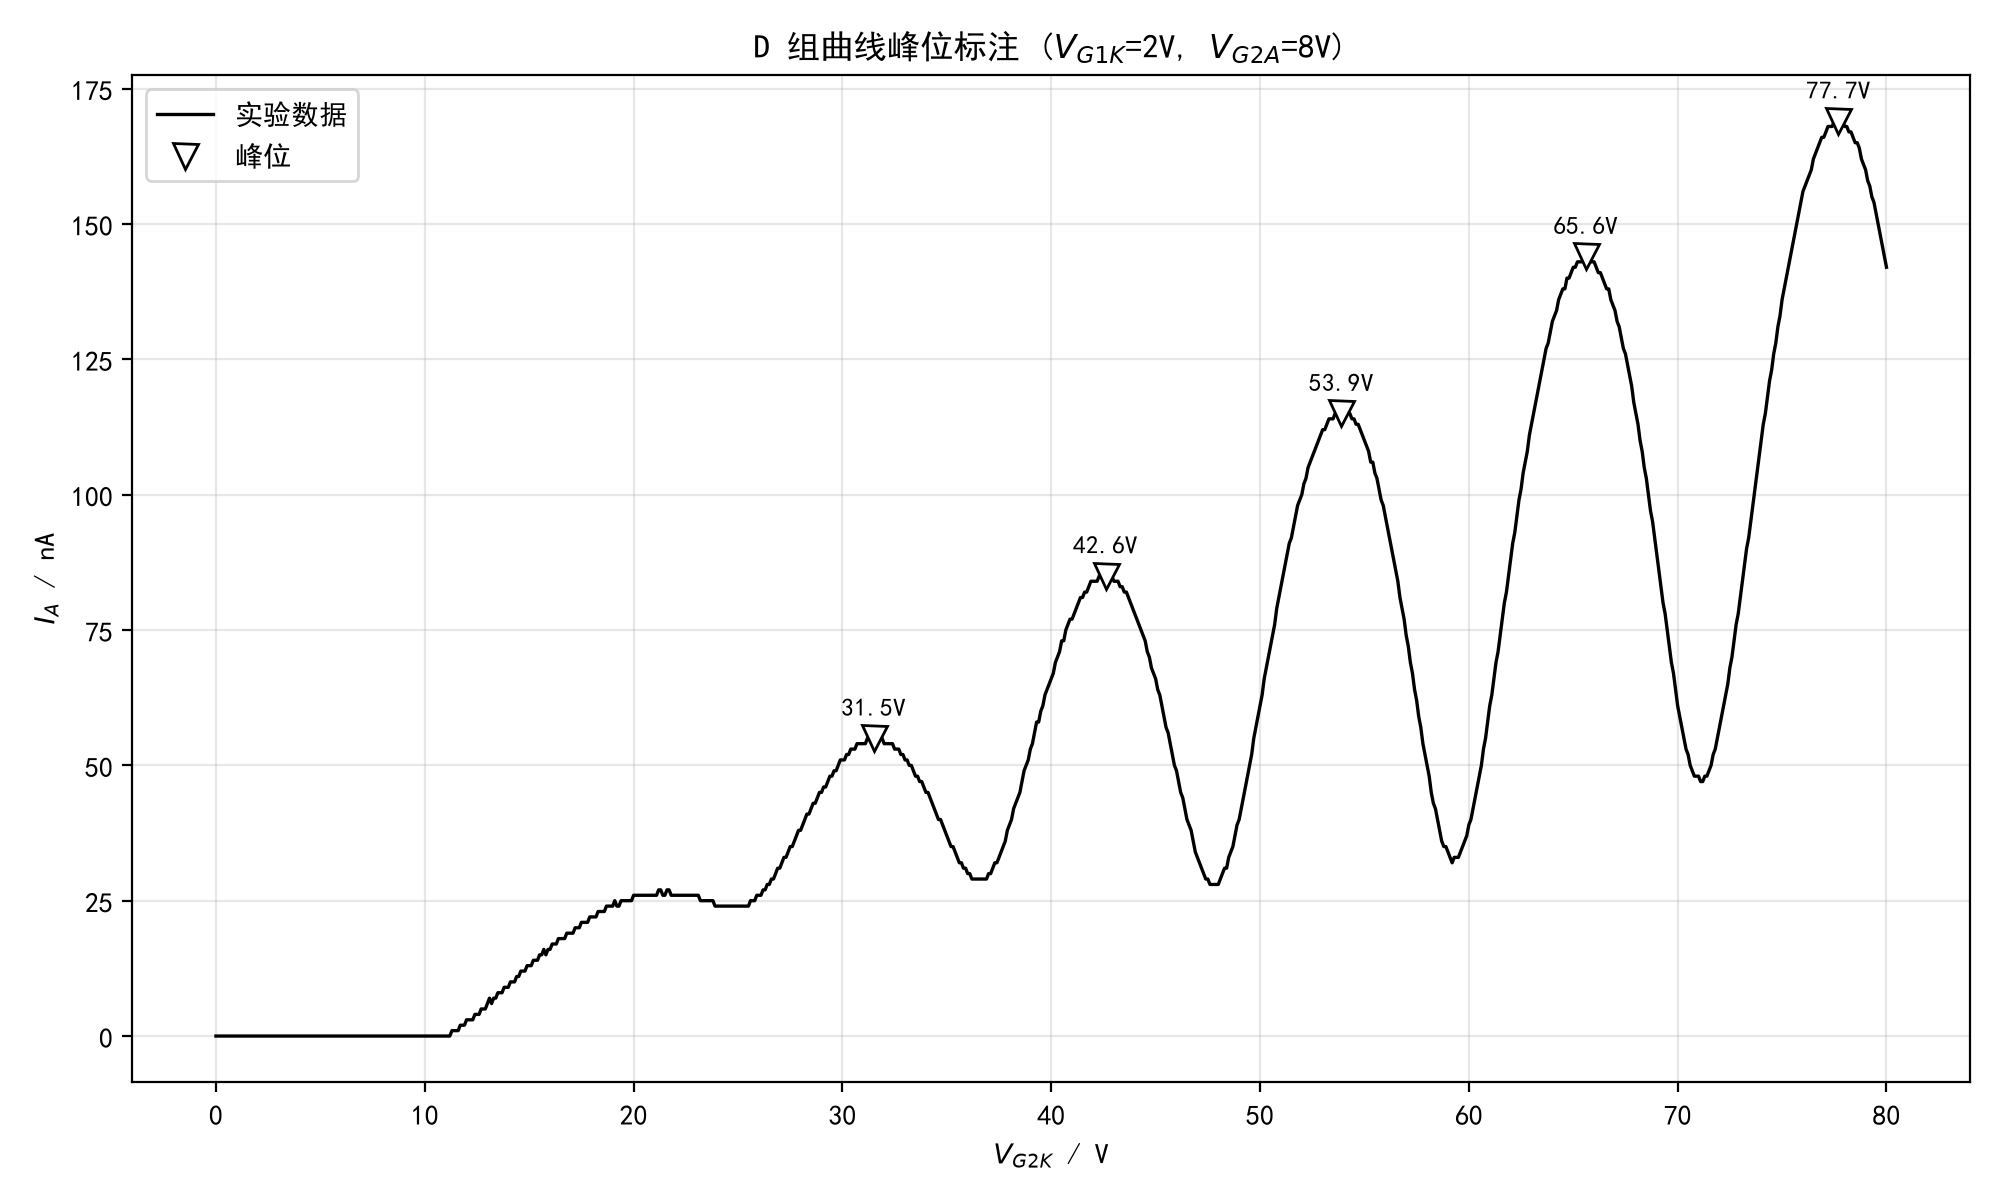
\includegraphics[width=0.9\textwidth]{frank_hertz_peaks.png}
    \caption{D 组曲线峰位标注（$V_{G1K}=\SI{2}{V}$，$V_{G2A}=\SI{8}{V}$）}
    \label{fig:peaks}
\end{figure}

\section{数据处理——逐差法}

\subsection{逐差法原理}

各峰位满足 $U_n = U_1 + (n-1)\Delta U$。若只用相邻峰差 $\Delta U_n = U_{n+1}-U_n$，每个差值只用到两个数据且不能充分利用测量范围；\textbf{逐差法}将相隔 $k$ 项的数据相减再除以 $k$：
\begin{equation}
    \Delta U^{(k)}_j = \frac{U_{j+k} - U_j}{k}, \qquad k = 2,\ 3,\ \dots
\end{equation}
本实验每组 5 个峰，取 $k=2$ 与 $k=3$，每组得到 6 个独立估计：
\begin{itemize}
    \item $k=2$：$(U_3-U_1)/2$，$(U_4-U_2)/2$，$(U_5-U_3)/2$
    \item $k=3$：$(U_4-U_1)/3$，$(U_5-U_2)/3$
\end{itemize}
（$U_5-U_1$ 与上列估计线性相关，不重复计入。）

\subsection{逐差计算结果}

以平均峰位为例，演示一组计算：
\begin{align}
    \frac{U_3-U_1}{2} &= \frac{53.75-31.42}{2} = \SI{11.17}{V}, &
    \frac{U_4-U_2}{2} &= \frac{65.42-42.37}{2} = \SI{11.52}{V}, \notag \\[2pt]
    \frac{U_5-U_3}{2} &= \frac{77.48-53.75}{2} = \SI{11.87}{V}, &
    \frac{U_4-U_1}{3} &= \frac{65.42-31.42}{3} = \SI{11.33}{V}, \notag \\[2pt]
    \frac{U_5-U_2}{3} &= \frac{77.48-42.37}{3} = \SI{11.70}{V}. \notag
\end{align}

6 组共 $6\times 6 = 36$ 个逐差估计值，汇总于表~\ref{tab:zhucha}。

\begin{table}[htbp]
    \centering
    \caption{各组逐差估计值（单位：V）}
    \label{tab:zhucha}
    \begin{tabular}{c c cc}
        \toprule
        组别 & 6 个逐差估计值 & 均值 / V & 标准差 / V \\
        \midrule
        A & 11.00, 11.45, 11.90, 11.20, 11.70, 11.45 & 11.450 & 0.326 \\
        B & 11.10, 11.55, 11.85, 11.30, 11.70, 11.48 & 11.496 & 0.270 \\
        C & 11.20, 11.60, 11.85, 11.33, 11.77, 11.53 & 11.546 & 0.249 \\
        D & 11.20, 11.50, 11.90, 11.37, 11.70, 11.55 & 11.536 & 0.246 \\
        E & 11.30, 11.45, 11.85, 11.43, 11.63, 11.58 & 11.540 & 0.191 \\
        F & 11.20, 11.60, 11.85, 11.37, 11.73, 11.53 & 11.546 & 0.238 \\
        \bottomrule
    \end{tabular}
\end{table}

合并全部 36 个估计：
\begin{equation}
    \overline{\Delta U} = \frac{1}{36}\sum_i \Delta U_i = \SI{11.52}{V}
\end{equation}

\subsection{不确定度评定（A 类）}

样本标准差：
\begin{equation}
    s = \sqrt{\frac{1}{35}\sum_i \left(\Delta U_i - \overline{\Delta U}\right)^2} = \SI{0.24}{V}
\end{equation}
平均值的标准不确定度：
\begin{equation}
    u_A(\Delta U) = \frac{s}{\sqrt{36}} = \SI{0.04}{V}
\end{equation}
电压读数误差 $\pm\SI{0.05}{V}$ 对应的 B 类分量 $u_B \approx \SI{0.02}{V}$，合成后 $u_C \approx \SI{0.05}{V}$，故最终结果表示为
\begin{equation}
    \boxed{\Delta U = (11.52 \pm 0.05)\ \mathrm{V}}
\end{equation}

\subsection{与参考值比较}

相对误差：
\begin{equation}
    E_r = \frac{|11.52 - 11.55|}{11.55}\times 100\% = 0.27\%
\end{equation}
在参考值 $\SI{11.55}{eV}$ 的不确定度范围内符合得很好。

\subsection{线性拟合验证（辅助方法）}

将各峰位电压对峰序号 $n$ 作最小二乘拟合 $U_n = a + b\,n$，斜率 $b$ 即为激发电位的另一独立估计，结果见图~\ref{fig:fit}。6 组曲线拟合斜率为 11.45--\SI{11.55}{V}（平均 \SI{11.52}{V}），与逐差法结果完全一致；平均峰位拟合残差均小于 \SI{0.4}{V}，说明 $U_n$--$n$ 线性关系良好，逐差法的前提成立。

\begin{figure}[htbp]
    \centering
    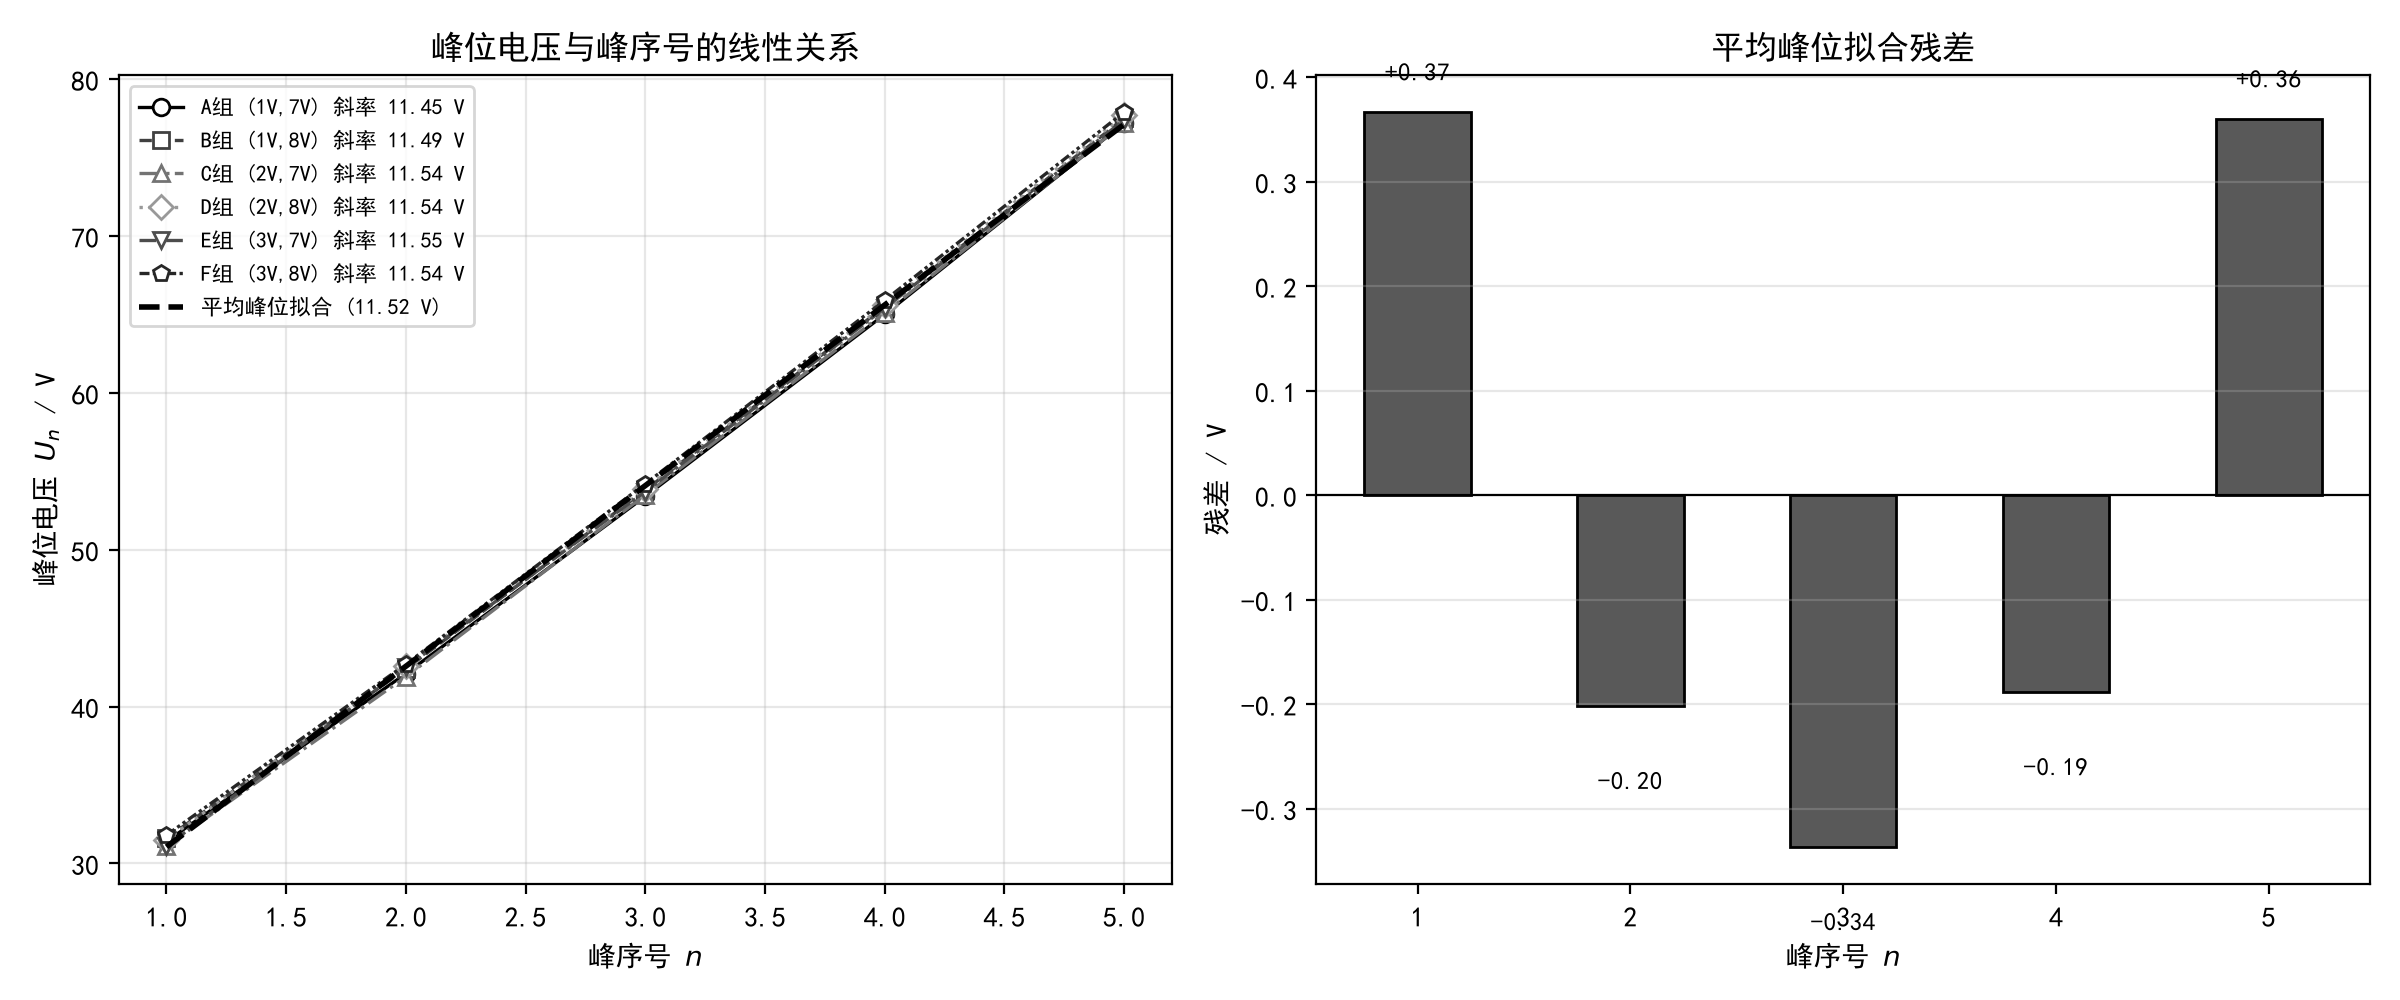
\includegraphics[width=\textwidth]{frank_hertz_linear_fit.png}
    \caption{峰位线性拟合与残差}
    \label{fig:fit}
\end{figure}

\section{结果与讨论}

\begin{enumerate}
    \item \textbf{测量结果}：氩原子第一激发电位 $\Delta U = (11.52 \pm 0.05)$ V，与参考值 \SI{11.55}{eV} 的相对偏差仅 0.27\%。实验直接证实了原子只能吸收确定份额的能量（$eU_0$），即原子能级的量子化。

    \item \textbf{工作参量对波形的影响}（对比 6 组曲线）：
    \begin{itemize}
        \item \textbf{拒斥电压 $V_{G2A}$} 越大（\SI{8}{V} vs \SI{7}{V}），到达板极的电子需克服的势垒越高，谷位电流更小、峰谷对比度更好，波形更清晰；
        \item \textbf{第一栅压 $V_{G1K}$} 主要影响阴极附近的空间电荷分布：$V_{G1K}$ 从 \SI{1}{V} 增至 \SI{3}{V}，峰位略向高电压方向移动（第一峰从 \SI{31.4}{V} 移至 \SI{31.8}{V}），峰高总体增大，但 $V_{G1K}$ 过大（\SI{3}{V}）时低电压段的本底电流明显抬升；
        \item 各曲线的峰间距在 11.45--\SI{11.58}{V} 之间，差别远小于峰位本身的差别，说明 $\Delta U$ 是管内气体的本征参量，与工作电压的选择基本无关。
    \end{itemize}

    \item \textbf{曲线起始段（0--\SI{12}{V} 电流为零、12--\SI{24}{V} 的台阶）}：加速电压低于约 \SI{12}{V} 时电子无法到达板极（动能不足以克服拒斥场），电流为零；随后电流上升并在 20--\SI{24}{V} 附近出现台阶，这是阴极与 $G_1$ 之间加速区段造成的电子能量分组现象，属正常现象，不影响峰间距测量。

    \item \textbf{误差来源分析}：
    \begin{itemize}
        \item 峰位判读误差（电压步距 \SI{0.1}{V}，平滑与寻峰引入约 $\pm 0.1$--\SI{0.2}{V} 的不确定度）——本实验主要的 A 类误差来源；
        \item 灯丝电压、拒斥电压的微小漂移导致峰位缓慢移动（对比 C 组与 D 组：仅 $V_{G2A}$ 改变 \SI{1}{V}，各峰移动约 0.1--\SI{0.4}{V}，但间距几乎不变，说明逐差/拟合方法能有效抵消系统漂移）；
        \item 管内氩气压强、温度的波动会引起自由程分布变化，使峰形展宽、峰位弥散；
        \item 接触电势差使第一峰位置偏离 $n=1$ 的线性外推值（拟合截距约 \SI{20}{V} 而非 \SI{11.55}{V}），这是夫兰克-赫兹管的固有效应，采用逐差法取间距而非绝对峰位正好消除了这一系统误差。
    \end{itemize}

    \item \textbf{结论}：逐差法充分利用了全部测量数据、扩大了电压差取值范围，有效抑制了缓慢漂移和零点偏移等系统误差。本实验测得氩原子第一激发电位为 \textbf{11.52 V}，与公认值 \SI{11.55}{eV} 在误差范围内一致，验证了玻尔原子能级量子化理论。
\end{enumerate}

\end{document}
